% !TeX spellcheck = fr_FR
\documentclass[11pt,a4paper,oneside]{report}
\usepackage[hmargin={1.25in,1.25in},vmargin={1.25in,1.25in}]{geometry}
%%%%%%%%%%%%%%%%%%%%%%%%
\setlength{\parindent}{0cm}
\makeindex
\usepackage{textcomp}
\usepackage{fancyhdr}
\usepackage{makeidx}
\pagestyle{myheadings}
\fancyhf{}
\rhead[\leftmark]{thepage}
%%%%%%%%%%%%%%%%%%%%%%%%
%\usepackage{natbib}
\usepackage[T1]{fontenc} % pour taper les lettres accentuées
%\usepackage[latin1]{inputenc}
\usepackage[UTF8]{inputenc}
\usepackage[francais]{babel}
\usepackage{url}
\usepackage{graphicx}
\usepackage{hyperref}
\usepackage{tikz}
\usepackage{pgfgantt} %draw timechart
\usepackage{amssymb, bm}
\newtheorem{mydef}{Définition}
\newtheorem{mytheorem}{Théorème}
\newtheorem{mylemme}{Lemme}

\begin{document}
%%%%%%%%%%%%%%%%
%\frontmatter
\begin{titlepage}


\begin{center}
\textbf{UNIVERSITÉ LIBRE DE BRUXELLES}\\
\textbf{Faculté des Sciences}\\
\textbf{Département d'Informatique}
\vfill{}\vfill{}

%\begin{center}
{\Huge  Implementing a Dynamic and Global Scheduling Algorithm  \vspace*{.5cm}  \linebreak[4] in a Real-Time OS}
%\end{center}

{\Huge \par}
\begin{center}{\LARGE Arabella Brayer}\end{center}{\Huge \par}

\vfill{}

\begin{figure}[h]
	\begin{center}
	\includegraphics[width=3cm]{img/sceauquadri}
	\label{fig:sceauquadri}
	\end{center}
\end{figure}
\vfill{}



\begin{flushright}{\large \textbf{Promoteur : Joël Goossens}}\hfill{}{\large Travail préliminaire au mémoire}\\
{
%	 \large Prof. Prénom Nom
 }\hfill{}{\large Master 1}\\
\hfill{}{\large Science de l'informatique}\end{flushright}{\large\par}
\vfill{}\vfill{}\enlargethispage{3cm}
\textbf{Academic year 2016~-~2017}
\end{center}
\end{titlepage}
\newpage
\thispagestyle{empty} 
\null

\newenvironment{vcenterpage}
{\newpage\thispagestyle{empty} 
\vspace*{\fill}}
{\vspace*{\fill}\par\pagebreak}

%\newpage
%\thispagestyle{empty}
%\vspace*{5cm}

%\begin{quotation}
%\noindent ``\emph{
%	%TODO choose a quotation
%	Vous pouvez aussi inclure une ou plusieurs citations générales en rapport avec votre sujet.
%}''
%\begin{flushright}\textbf{l'auteur (vrai ou supposé), date}\end{flushright}
%\end{quotation}

%\medskip
%
%\begin{quotation}
%\noindent ``\emph{Il existe des compilations de telles citations.}''
%\begin{flushright}\textbf{autre auteur, date}\end{flushright}
%\end{quotation}
%\chapter*{Remerciements}
%\thispagestyle{empty} 

%\noindent Je tiens à remercier ... 

%\medskip
%sans oublier les plus importants, exercice parfois délicat
\thispagestyle{empty} 
\setcounter{page}{0}
\tableofcontents
%\mainmatter 

%%%%%%%%%%%%%%%%%%%%%%%%%%%%%%%%%%%%%%%%%%%%%%%%%%%%%%%%%%%%%%%%%%%%%%%%%%%%%%%%%%%%
%%%%%%%%%%%%%%%%%%%%%%%%%%%%%%%%%%%%%%%%%%%%%%%%%%%%%%%%%%%%%%%%%%%%%%%%%%%%%%%%%%%%
%%%%%%%%%%%%%%%%%%%%%%%%%%%% INTRODUCTION %%%%%%%%%%%%%%%%%%%%%%%%%%%%%%%%%%%%%%%%%%
%%%%%%%%%%%%%%%%%%%%%%%%%%%%%%%%%%%%%%%%%%%%%%%%%%%%%%%%%%%%%%%%%%%%%%%%%%%%%%%%%%%%


% chapitre introduction

% TODO trouver meilleur nom qu'introduction, l'introduction est une partie de cette première partie.
\chapter{Introduction}{}
\setcounter{page}{1}


\section{Présentation générale du sujet}
%TODO il FAUT parler des objectifs en terme de réduction de consommation.
%TODO c'est MON dada. 

Dans le paysage quotidien des appareils informatiques, il existe toujours plus de systèmes embarqués. 
Parmi eux, un nombre très important de systèmes temps réel qui nécessitent des 
ordonnanceurs adaptés. Ce champ de recherche a été largement nourri durant les 
vingt dernières années par de nombreuses publications scientifiques. \\

Les systèmes embarqués n'ont pas toujours de grands besoins en efficacité, 
ils doivent principalement être sûrs, et réactifs. 
Toutefois, un système dont l'efficacité n'est pas maximale n'utilise pas ses ressources 
de façon optimale. 
De nos jours où la gestion énergétique se doit d'être la plus économe possible, 
où l'on est de plus en plus exigeant concernant l'efficacité, il est envisageable que 
la solution évolue du côté des industries.\\

Par ailleurs, cela fait plusieurs années que la croissance de l'efficacité des appareils n'est plus 
principalement due à des améliorations physiques des composants. 
En effet, la multiplication des processeurs dans les ordinateurs a permis
de paralléliser les exécutions, et c'est ainsi que la quasi stagnation des 
technologies a pu être contournée pour continuer la progression.
% TODO add ref du cours de micro


Le monde des systèmes embarqués en temps réel a bénéficié de ces améliorations, 
et dispose également de processeurs multi-c\oe{}urs. Cependant, leur gestion n'est 
à l'heure actuelle pas optimale, la plupart des systèmes sont  
gérés soit comme des systèmes mono-processeurs, soit avec des algorithmes partitionnés \cite{paolillo_new_nodate}. 
Dans le premier cas, les ressources ne sont pas utilisées de façon optimale, 
et dans le second, des implémentations et tests ont montré empiriquement 
que les algorithmes globaux pouvaient présenter des avantages intéressants, comme 
une meilleure répartition de l'utilisation des processeurs \cite{baker_analysis_2005}. 
\\ 

Le décalage entre la connaissance scientifique et les implémentations réelles 
peut s'expliquer en partie par le fait qu'il soit compliqué de gérer le partage des ressources, 
et que cette complexité n'apporte pas suffisamment d'avantages à l'heure qu'il est.\\

Le fait que l'industrie n'implémente pas à ce jour de solutions plus "performantes" 
pour les systèmes embarqués pose plusieurs problèmes :
\begin{enumerate}
	\item Le matériel n'est pas exploité de façon optimale.
	\item Par conséquent, on utilise bien plus d'énergie que nécessaire. 
	À l'heure actuelle, dans un monde où l'on cherche à consommer le moins possible, 
	cela pose question. Mais au delà, cela signifie également plus de maintenance 
	sur ces appareils parfois sans source de renouvellement d'énergie.
	\item Certains systèmes embarqués nécessitent une très basse consommation car 
	ils sont difficiles d'accès ou non faciles à recharger.
\end{enumerate}

Toutes ces raisons poussent à s'intéresser à une implémentation réelle et réaliste 
d'ordonnanceurs connus dans la littérature, mais moins dans la réalité.

C'est dans ce contexte que s'inscrit ce travail d'implémentation d'un ordonnanceur en temps réel 
global et multiprocesseur, dont un des objectifs est d'améliorer la connaissance pratique 
d'ordonnanceurs multiprocesseurs globaux, d'en apercevoir les limites. 
Cette implémentation pourrait amener plusieurs résultats intéressants : \\
\begin{itemize}
	\item Une comparaison entre des résultats théoriques et l'effet de leur mise 
	en \oe{}uvre
	\item L'origine de ces différences
	\item Vérifier les avantages, inconvénients ou obstacles à la 
	commercialisation de telles solutions.
\end{itemize}

\section{Contexte et objectifs}

%\subsection{Limites du parallélisme}
%Le parallélisme a montré ses limites, connues depuis longtemps dans la littérature scientifique. 
%Par exemple, la loi d'\href{https://en.wikipedia.org/wiki/Amdahl\%27s_law}{Amdahl} montre 
%l'accélération théorique que l'on peut atteindre en améliorant certains paramètres : 
%%TODO mettre une référence correcte
%\begin{itemize}
%    \item La portion de code exécutable en parallèle (tout un programme séquentiel ne peut pas forcément 
%    être parallélisable)
%    \item Le nombre de processeurs. 
%\end{itemize}
%On remarque alors que le nombre de processeurs n'influence la vitesse d'exécution que jusqu'à une certaine limite 


\subsection{Ordonnanceurs globaux}
Comme il sera expliqué plus tard dans ce document, il existe deux grandes familles d'ordonnanceurs 
multiprocesseur :\\
\begin{itemize}
	\item Les ordonnanceurs partitionnés
	\item Les ordonnanceurs globaux
\end{itemize}
Si parmi ces deux familles d'ordonnanceurs, les systèmes mono-processeurs, voire 
partitionnés ont le plus de succès auprès de l'industrie, 
ce n'est pas la famille la plus efficace pour tout type de classe de tâches. 
Les algorithmes globaux répartissent habituellement mieux l'utilisation des processeurs, 
les migrations sont possibles et donc les temps de réalisation sont généralement moins grands.
\\ % TODO add ref ?... J'ai une conf, mais pas un papier scientifique...
% http://retis.sssup.it/~giorgio/slides/cbsd/mc3-global-2p.pdf


En 1988, Hong and Leung \cite{hong_-line_1988} publient un article dans lequel est 
démontré que : \\
\textit{"For every m > 1, no optimal on-line scheduler can exist for task systems with two or more distinct deadlines"} : 
\textit{Il n'existe pas d'ordonnanceur multiprocesseur en ligne optimal pour un système de tâches 
avec plusieurs échéances distinctes}, donc un système de tâches dites "sporadiques".

Or, les systèmes embarqués doivent très souvent exécuter des systèmes de tâches sporadiques, 
cela tient de leur nature : la plupart d'entre eux attendent en effet de recevoir des 
signaux, qui arrivent de façon indéterminée.

Toutefois, des publications ultérieures viennent compléter cette preuve, et démontrent 
que des ordonnanceurs globaux optimaux existent, mais nécessitent de la clairvoyance.
%TODO add ref gossens




\subsection{HIPPEROS}
\textbf{HIPPEROS} (High Performance Parallel Embedded Real-time Operating Systems)
est un \textbf{RTOS} développé depuis plusieurs années par une spinoff de l'ULB.
Il bénéficie des connaissances apportées par le monde de la recherche dans 
le domaine des systèmes critiques avec multic\oe{}urs. Une de ses particularités 
est sa modularité, qui permet d'adapter ses possibilités en fonction du système 
lors de la compilation de l'OS, ainsi peut-on différencier deux installations 
en fonction des particularités.

\textbf{HIPPEROS} est un candidat idéal pour l'implémentation d'un ordonnanceur 
global, mais une partie du travail consistera à tirer parti de ses particularités. 
Par exemple, ce système d'exploitation gère les c\oe{}urs en leur attribuant des 
niveaux différents. L'un est considéré comme "maître" et les autres comme "esclaves". 
Ceci peut apporter un comportement particulier, ce auquel il convient d'apporter 
l'attention nécessaire. En résumé, une nouvelle implémentation sur un OS différent 
peut elle-aussi apporter à la connaissance générale des détails importants.


\section{Problématique}
L'ordonnanceur idéal -- c'est à dire optimal pour toute classe de tâches et 
qui ne fasse pas de multiples migrations coûteuses n'existant pas, 
notre sujet est de sélectionner l'un d'eux parmi une liste 
d'ordonnanceurs connus (ne serait-ce que dans la littérature) afin que cela apporte 
à la connaissance générale, tant sur le plan théorique que pratique.

Par ailleurs, certains des ordonnanceurs présentés dans l'état de l'art 
 ont déjà bénéficié d'une implémentation sur un \textbf{RTOS}, et une nouvelle 
 implémentation sur un \textbf{OS} différent pourrait apporter un éclairage intéressant quant 
 aux différences de comportements.
Dans certaines présentations d'ordonnanceurs sont proposées des hypothèses à propos du comportement, 
comme faire globalement plus de préemption, de migrations. 
Le comportement observé dans des conditions différentes pourrait être vérifié, ou le contraire.

La question cruciale de cette première partie de travail 
consiste donc à faire un tour d'horizon de la littérature afin de pouvoir 
sélectionner un ordonnanceur pertinent à implémenter sur le \textbf{RTOS} \textbf{HIPPEROS}.

\section{Vocabulaire général sur les systèmes temps réel}

\subsection{Système de tâches}
Un système de tâches et un ensemble de tâches ayant les mêmes propriétés devant être exécutées. 

\subsection{Tâche (temps réel)}
Une tâche correspond à une sorte de programme, c'est à dire une série d'instructions 
qui doivent être exécutées par un processeur. 
Il y a plusieurs caractéristiques 
et propriétés qui définissent une tâche, que nous allons définir ici : 
\begin{itemize}
    \item[\textbf{Temps de réalisation}] : C'est le moment $t$ où une tâche $\tau$ peut commencer à être exécutée.
    \item[\textbf{Début, Fin}] : Le moment où la tâche commence effectivement à être exécutée, ou termine son exécution.
    \item[\textbf{Temps de réponse\label{Response Time}}] : Temps maximum nécessaire à la réalisation de la tâche 
    entre le temps de réalisation et Fin. %TODO vérif
    \item[\textbf{Échéance, temps limite}] : Correspond au temps limite au delà duquel la tâche doit avoir été exécutée. Il existe deux types d'échéances : 
    une absolue, et une relative. L'échéances relative est une valeur fixe qui 
    est une propriété de la tâche, elle dépend donc du temps de réalisation.\\
    L'échéances absolue quant à elle est calculée avant l'exécution, et correspond 
    à un temps $t$ absolu.%TODO explain better, relire cours ptete ?!
    
    \item[\textbf{Worst Case Execution Time}] Afin de faciliter les calculs et l'abstraction du problème, l'on pose habituellement que le temps considéré d'exécution de 
    la tâche est le pire temps. Cela permet d'envisager le pire scénario, et ainsi 
    de s'assurer que si celui-ci est possible, alors dans de meilleures conditions, 
    la faisabilité est conservée. La notation utilisée dans le reste de ce document 
    est  \textbf{WCET} : \textbf{W}orst \textbf{C}ase \textbf{E}xecution \textbf{T}ime
    
    \item[\textbf{Laxité}] La laxité d'une tâche est la durée entre sa réalisation et son échéance. 
    Pour une tâche $\tau_i$, la laxité est :
    \begin{center}
        $L_i = D_i - C_i$
    \end{center}
    \vspace{0.5cm}
    \item[\textbf{Tâches périodiques}]
    Une tâche périodique est une tâche qui génère régulièrement des jobs.  
    Formellement, une tâche périodique est définie par un 4-uplet $(O, T, D, C)$ où 
    \begin{itemize}
        \item[O] est l'"offset", c'est à dire le temps que met la tâche à générer un premier job.
        \item[T] est la période, c'est à dire le temps qui sépare deux générations de job par la tâche. 
        Comme le premier job est généré à l'instant $O$, alors $\forall i \in \{0, \infty \} t = O + i\times T$ 
        où $t$ est le temps où la tâche est générée la $i$ème fois.
        \item[D] est l'échéance relative, c'est à dire le temps qui sépare au maximum la génération 
        d'un job et sa réalisation.
        \item[C] est le temps de réalisation. Dans les algorithmes, on utilise -- comme expliqué précédemment -- le \textbf{WCET}.
    \end{itemize}	
    Dans le cas de tâches périodiques, on distingue trois cas différents : \\
    \begin{enumerate}
        \item si l'échéance est égale à la période $\forall \tau_i, D_i = T_i$ : tâche à \label{echeancesurrequete}échéance sur requête
        \item si l'échéance est inférieure ou égale à la période $\forall \tau_i, D_i \leq T_i $ , on dit que la tâche est à \label{echeancecontrainte} échéance contrainte
        \item s'il n'y a pas de contrainte particulière, la tâche est dite "à échéance arbitraire".
    \end{enumerate}
    Les solutions d'ordonnancement pour ces trois types de tâches diffèrent donc. 
    Globalement, on peut ordonner ces trois types de tâches : \\
    échéance sur requêtes $\subset$ échéance contrainte $\subset$ échéance arbitraire.
    
    \item[\textbf{Tâche sporadique}] : Une tâche sporadique est une tâche qui génère de nouveaux jobs, 
    comme dans le cas de la tâche périodique. 
    La différence entre ces deux types est que la tâche sporadique 
    génère deux jobs avec un intervalle de temps au moins égal à la durée correspondant à sa période, 
    et pas exactement égal. Les systèmes embarqués ont souvent des tâches sporadiques à gérer : 
    en effet, un système qui est composé de capteur aura du mal à prévoir l'arrivée d'un signal de 
    celui-ci. 
    
    \item[\textbf{Tâche apériodique}] : Pour ce type de tâches, on ignore la régularité de 
    l'arrivée de nouveaux jobs. Les propriétés du job ne sont connues que lorsqu'un job est 
    généré dans le système.
    
\end{itemize}

\subsection{Job}
Un job est une instance d'une tâche. 
\subsection{RTOS}
(Real Time Operating System) Système d'Exploitation Temps Réel.\\
Un système d'exploitation Temps Réel un système d'exploitation implémenté pour les systèmes 
à temps réel, c'est à dire dont l'objectif est d'assurer le respect de certaines échéances. 

Cela concerne pour beaucoup les systèmes dits "critiques", c'est à dire dont la sécurité 
est primordiale (avions, centrales nucléaires, pacemakers, etc.). Ce type de dispositifs 
est actuellement très répandu, notamment dans les voitures.\\
Les contraintes sont différentes de celles des systèmes d'exploitations traditionnels puisqu'on 
doit garantir le respect des échéances associées à chacune des tâches. 

Cependant, si les systèmes d'exploitation temps réel ont des besoins de respect des échéances, 
cela ne signifie pas qu'ils aient forcément de grands besoins en efficacité ou en rapidité, ce qui 
est primordial est que les échéances soient respectées. 
Pour certains systèmes critiques, on comprend qu'il soit important de pouvoir prouver 
minutieusement que le système est correct, et ne risque pas de produire des pannes, ce qui peut 
s'avérer très grave. \\
	
\subsection{Contraintes strictes, contraintes relatives} 
Dans le cas strict, le système doit impérativement respecter tous les temps limites. Aucun dépassement n'est toléré. Dans le cas des contraintes relatives, ce respect 
est moins impératif, et on pourra dépasser les délais occasionnellement. \\


\subsection{Ordonnanceur}
Un ordonnanceur (\textit{Scheduler}) est la partie logicielle de 
l'\textit{OS} chargée d'orchestrer l'ordre d'exécution des tâches du système 
selon des priorités fixées à l'avance ou durant l'exécution. 
On distingue trois types d'assignation de priorités des ordonnanceurs : \\
\begin{enumerate}
	\item Priorité fixée au niveau des tâches : Ce type d'ordonnanceur fixe la priorité 
	avant l'exécution, et celle-ci dépend donc des attributs de la tâche. 
	Deux exemples d'ordonnanceurs de ce type seront présentés plus loin : Rate Monotonic et 
	Deadline Monotonic.
	\item Priorité fixe au niveau des jobs : La priorité est fixée par l'ordonnanceur à l'arrivée du job 
	dans l'exécution, et elle ne peut pas changer jusqu'à la réalisation du job. Un exemple sera présenté plus loin : Earliest Deadline First.
	\item Priorité dynamique : L'ordonnanceur peut recalculer à tout moment de l'exécution 
	la priorité du job avec un exemple connu, Least Laxity First\cite{hutchison_predictability_2006}.
\end{enumerate}
	
Selon les cas, l'ordonnanceur peut avoir à gérer un seul processeur. Dans ce 
document, on parlera dans ce cas d'ordonnanceur mono-processeur. Toutefois, de plus en 
plus de systèmes possèdent plusieurs processeurs, et il existe deux grandes familles 
d'ordonnanceurs associés à ces systèmes : les Partitionnés, ou les Globaux. \\

\subsection{Work-Conservative} 
Un ordonnanceur peut-être "économe", ou "non-économe". Dans le premier cas, si le processeur est libre, 
et qu'une tâche est prête à être exécutée, l'ordonnanceur donnera l'instance : cela signifie 
qu'on évite les temps d'inactivité du processeur. Dans le second cas, une tâche ne sera pas toujours ordonnancée.
Dans le reste de ce document, les ordonnanceurs présentés sont tous économes selon cette définition.

\subsection{En ligne, hors ligne}
Un ordonnanceur en ligne fait ses opérations d'ordonnancement durant le runtime. 
Un ordonnanceur hors ligne fait des opérations au préalable. 
Un exemple pour illustrer cela est un ordonnanceur partitionné, qui aura partagé le système 
en sous-systèmes durant une phase hors-ligne, et un ordonnanceur global non clairvoyant qui 
ordonnance au fur et à mesure durant l'exécution. 

\subsubsection{Ordonnanceur multi-processeur Partitionné}
Un ordonnanceur partitionné composé de $n$ tâches et de $m$ processeurs divise 
le système en $m$ sous-systèmes qui seront ensuite ordonnancés par autant d'ordonnanceurs 
mono-processeurs. Le problème principal consiste à découper efficacement le système de tâches.

\subsubsection{Ordonnanceur multi-processeur Global}
Un ordonnanceur global ne sépare pas le système en sous-systèmes mais gère une 
queue de tâches prêtes à être exécutées. Ainsi à chaque instant où il devra prendre une décision 
d'ordonnancement, il devra ordonnancer toute la liste des $m$ processeurs.\\
Contrairement aux ordonnanceurs partitionnés, les migrations sont possibles. Le problème 
est donc de réduire leur nombre pour ne pas faire de mouvements inutilement.
	
\subsection{Préemption et hypothèse} 
Un système est dit préemptif s'il a la capacité 
	de mettre l'exécution d'un job en pause et d'exécuter un autre à la place. 
	Une hypothèse pour simplifier la question théorique des ordonnanceur est 
	très souvent faite dans la littérature : on considère le temps de 
	préemption comme nul. Cette hypothèse est bien entendu fausse, et il faudra 
	en tenir compte, particulièrement dans ce travail où l'on tente de faire 
	le lien entre la théorie et la mise en pratique. 

\subsection{Utilisation}
Le facteur d'utilisation $U_i$ d'une tâche périodique $\tau_i$ est le rapport entre 
son temps d'exécution et sa période. Par exemple, pour une tâche $\tau_i$ tel que 
$WCET = 50 ms$ et $T = 30 ms$, le processeur doit allouer $\frac{30}{50}$ du temps 
total d'exécution à cette tâche.\\

L'utilisation (ou le facteur d'utilisation) d'un système périodique est la proportion de temps 
passée par le processeur à l'exécution de tâches d'un système donné. 
Le calcul de l'utilisation permet dans certains cas et certaines conditions de donner une indication 
à propos de la faisabilité du système par un certain ordonnanceur. 
\\

Liu et Layland \cite{liu_scheduling_1973} en donnent une définition formelle dans leur article décrivant l'ordonnanceur \textbf{Rate Monotonic} (présenté plus tard dans ce document).\\ 

Soit $C_i$ le temps d'exécution d'une tâche $\tau_i$, et soit $T_i$ sa période, voici la définition de 
l'utilisation pour un système de $m$ tâches :\\
\begin{center}
	$U_{tot} = \sum_{i = 1}^{m}(\frac{C_i}{T_i})$
\end{center}

\subsection{Laxité}
%\ref{laxite}
La laxité d'un job est la durée entre son temps de réalisation et son échéance absolue. 
%todo add blabla


%%%%%%%%%%%%%%%%%%%%%%%%%%%%%%%%%%%%%%%%%%%%%%%%%%%%%%%%%%%%%%%%%%%%%%%%%%%%%%%%%%%%
%%%%%%%%%%%%%%%%%%%%%%%%%%%%%%%%%%%%%%%%%%%%%%%%%%%%%%%%%%%%%%%%%%%%%%%%%%%%%%%%%%%%
%%%%%%%%%%%%%%%%%%%%%%%%%%%% ETAT DE L'ART %%%%%%%%%%%%%%%%%%%%%%%%%%%%%%%%%%%%%%%%%%
%%%%%%%%%%%%%%%%%%%%%%%%%%%%%%%%%%%%%%%%%%%%%%%%%%%%%%%%%%%%%%%%%%%%%%%%%%%%%%%%%%%%


\chapter{État de l'art}

La littérature sur le sujet des ordonnanceurs est assez vaste. 
Ceux-ci sont composés principalement de trois grandes familles :\\
\begin{itemize}
	\item Les mono-processeurs
	\item Les multi-processeurs Partitionnés
	\item Les multiprocesseurs Globaux
\end{itemize}
Les ordonnanceurs mono-processeurs étant plus simples à appréhender, nous commencerons 
par présenter cette famille.

\section{Ordonnanceurs mono processeur}

\subsection{Rate Monotonic}
L'ordonnanceur \textbf{R}ate \textbf{M}onotonic (RM) est décrit par Liu et Layland \cite{liu_scheduling_1973} en 1973. C'est 
donc un ordonnanceur classique, bien connu, ainsi que largement documenté \cite{kermia_ordonnancement_2009}. 
L'idée de base est qu'une tâche avec une période courte évolue rapidement, et 
doit donc être prioritaire.\\
On considère un ensemble de tâches périodiques et indépendantes.
Les priorités sont statiques et attribuées en fonction de la durée de la période, ainsi 
la tâche avec la période la plus faible sera de priorité plus élevée. 
Un des points fondamentaux de l'article est la preuve de l'optimalité de RM dans le cas 
préemptif, à tâches périodiques, à échéance sur requête, indépendantes, simultanées.
Les auteurs énoncent même une condition suffisante de faisabilité pour un système à $m$ tâches : \\
\begin{center}
	$\sum_{i=1}^{m}\frac{C_i}{T_i} \leq m(2^{\frac{1}{m}}-1)$
\end{center}
Notons également que pour $n \rightarrow \infty$, $\sum_{i=1}^{m}\frac{C_i}{T_i} \leq m(2^{\frac{1}{m}}-1) \rightarrow \ln(2) \approx 0.69$.
Une condition suffisante est donc que le facteur d'utilisation du système soit inférieur à 0.69. 
Dans ce cas, le système est ordonnançable par RM.\\

Des améliorations ont par la suite été apportées par Joseph et Pandya \cite{joseph_finding_1986}.
qui ont trouvé une condition nécessaire et suffisante. 
Ainsi, si $RT(t_i)$ est le temps de réponse (\ref{Response Time}) d'une tâche $t_i$, 
alors si un ensemble de tâches périodiques est trié par ordre décroissant, l'équation suivante 
définit la borne supérieure du temps de réalisation :
\begin{center}
	$RT(t_i)^{q+1} = \sum_{j=1}^{i-1} \lceil \frac{RT(t_i)^q}{T(t_i)} \rceil \times C(t_j)) + C(t_i)$
\end{center}
Le système est ordonnançable si et seulement si $\forall i_{(1 \leq i \leq m)}RT(t_i) \leq T_i$.
On pourra résoudre récursivement cette équation afin de prouver sa faisabilité.\\

\textit{RM} n'est cependant optimal que pour cette classe de tâches. Dès que les propriétés changent, 
il faudra se tourner vers un autre type d'ordonnanceur.


\subsection{Deadline Monotonic}
Deadline Monotonic (DM) est un ordonnanceur pour les systèmes à départ simultanés ($offset = 0$) et 
à échéance contrainte\ref{echeancecontrainte}($D_i \leq T_i$). Il a été décrit par Leung et Whitehead 
\cite{leung_complexity_1982}. Cet article aborde le point de vue mono-processeur et multi-processeur partitionné, 
dont il sera question plus loin dans ce document.\\

Avec cet ordonnanceur, les priorités sont fixes, au niveau des tâches.
Plus l'échéance est petite, plus la priorité est élevée. On peut considérer que \textit{RM} est 
un cas particulier de \textit{DM}, puisque pour \textit{RM}, les tâches sont à échéance sur requête \ref{echeancesurrequete}.
Il n'existe pas de test de faisabilité basé sur l'utilisation du système. Pour vérifier celle-ci, 
il faut avoir recours à l'équation décrite plus haut. 
On peut la résoudre récursivement à l'aide de ce système d'équations: \\
\begin{enumerate}
	\item $W_0 = C_i $
	\item $W_{k+1} = C_i + \sum_{j = 1}^{i-1}\lceil \frac{W_k}{T_j} \rceil \times C_j $
\end{enumerate}



\subsection{Earliest Deadline First}
\textbf{E}arliest \textbf{D}eadline \textbf{F}irst (EDF) est un ordonnanceur 
qui a été introduit en 1973, à la même période que Rate Monotonic, également 
par Lui et Layland \cite{liu_scheduling_1973}. C'est un ordonnanceur à départ différé ($Offset \neq 0$) 
et à échéance arbitraire (pas de contrainte sur l'échéance par rapport à la période), 
qui fixe les priorités sur les jobs. L'assignation de la priorité se fait sur base de 
la proximité de l'échéance absolue : Plus cette échéance est proche et plus la priorité est élevée. 
Une façon déterministe et arbitraire de régler les cas d'égalité doit être décidée.\\

\textit{EDF} est optimal pour toutes les tâches synchrones et asynchrones, avec et sans 
contraintes sur les échéances. 
Cela signifie que si un système est ordonnançable, \textit{EDF} peut l'ordonnancer.\\
Cette propriété est importante, car les classes de tâches ordonnancées par \textit{EDF} 
sont plus larges que \textit{RM} et \textit{DM}, par conséquent, \textit{EDF} peut ordonnancer également les 
mêmes classes qu'\textit{RM} et \textit{DM} en conservant son optimalité. \\

Les tests de faisabilité avec \textit{EDF} dépendent de la classe de tâche considérée. 
Pour un système synchrone et à échéance sur requête, 
une condition nécessaire et suffisante de faisabilité est donc que l'utilisation soit inférieure 
à 100\%, c'est à dire : \\
\begin{center}
	$\forall \tau_i \in \Gamma_m, \sum_{i=1}^{m}\frac{C_i}{T_i} \leq 1 $
\end{center}

Dans le cas d'un système synchrone à échéance arbitraire, on doit considérer un intervalle de 
recherche $[0, L]$ avec $L$ qui peut se calculer de façon itérative en cherchant un point fixe 
avec cette formule : \\
\[
\left \{
\begin{array}{r l}
W_0 &= \sum_{i = 1}^{m}C_i\\
W_{k+1} & =\sum_{i = 1}^{m} \lceil \frac{W_k}{T_i} \rceil \times C_i
\end{array}
\right.
\]

Dans le cas des systèmes de tâches asynchrones, l'intervalle considéré est plus grand : 
$[0, O_{max} + 2 \times P]$ avec $O_{max}$ l'offset maximum du système et 
$P$ le plus petit commun multiple ($ppcm$) de toutes les périodes du système, soit : \\
\begin{center}
	$P = ppcm\{T_i | i \in \{1, ... m\}\}$
\end{center}

Malgré le fait que la littérature montre la supériorité d'\textit{EDF} sur \textit{RM}, 
il semble que ce soit RM qui soit plus volontiers choisi pour implémentation. 
Sa réputation est qu'il est plus simple. 
On trouve un résumé du débat qui existe à ce sujet dans un article de Buzzato
\cite{buttazzo_rate_2005}.

\section{Multi-processeurs : les différentes familles d'ordonnanceurs}
% TODO !! 2 types de pb : bin packing ou search :
% todo see http://www.irisa.fr/alf/downloads/puaut/STR/STRmulticore.pdf
%TODO revoir cours de goossens
Dans la partie précédente, nous avons présenté certains algorithmes mono-processeur, 
ainsi que quelques conditions d'ordonnançabilité.
De nos jours, une grande partie des architectures employées dans les systèmes embarqués 
est multiprocesseur. 
Les stratégies mises en place pour l'ordonnancement de tels 
systèmes sont différentes. Dans la littérature, il est habituel de présenter 
deux familles principales d'ordonnanceurs multi-processeurs :\\
\begin{itemize}
	\item Les ordonnanceurs partitionnés
	\item Les ordonnanceurs globaux
\end{itemize}
Nous verrons qu'une troisième famille est souvent présentée également. Elle représente un 
mélange des deux précédentes. On parle d'ordonnanceurs \textit{hybrides}, ou \textit{semi-globaux}.

\section{Les ordonnanceurs partitionnés}
L'idée principale derrière la stratégie du partitionnement est que pour tout 
ensemble $\Gamma$ de $n$ tâches, si l'utilisation de chaque tâche est inférieure à $1$, 
alors il existe un ordonnanceur de $m <= n$ processeurs capable d'ordonnancer cet ensemble. 
Il y a principalement deux optiques différentes pour envisager ce problème : \\
\begin{itemize}
	\item Partir de l'ensemble maximum et appliquer un algorithme de recherche afin de trouver 
	la valeur de $m$ la plus petite telle que l'ordonnancement soit possible
	\item Résoudre ce problème connu dans la littérature comme celui du Bin-Packing, 
	et rejoindre un domaine bien connu et largement documenté.
\end{itemize}
Dans la suite du document, on ne s'intéressera qu'aux heuristiques liées au Bin-Packing et 
laisserons de côté les algorithmes de recherche.

\subsection{Ordonnanceurs à priorité fixe sur tâche}

La stratégie de partitionnement consiste à diviser l'ensemble de tâches en sous-ensembles qui seront 
attribués à un processeur particulier. Cela permet de conserver les mêmes algorithmes ainsi 
que tests d'ordonnançabilité que ceux 
décrits précédemment puisqu'en divisant le système en sous-systèmes attribués à un 
processeur chacun, cela revient à appliquer "localement" une stratégie mono-processeur, contre 
une stratégie globale multi-processeur \cite{ndoye_ordonnancement_2014}.
%TODO add formal def

Concrètement, cela revient à diviser un ensemble $\Gamma$ de tâches en $n$ sous-ensembles 
$\gamma \in \Gamma$ et d'attribuer à chacun des $m$ processeurs un de ces sous-ensembles $\gamma$.\\


Le problème du partitionnement consiste donc en premier lieu 
à résoudre une division du système en sous-systèmes, ce qui est connu dans la 
littérature scientifique comme le problème du bin-packing \cite{ausiello_approximation_1984}.
Ce problème est $NP$ difficile, si bien qu'en pratique, 
des heuristiques sont appliquées, comme par exemple :\\
\begin{itemize}
	\item First-fit 
	\item Best-fit
	\item Next-fit
\end{itemize}

Plusieurs algorithmes de ce type ont été présentés dans la littérature scientifique
dans les années 80 comme par exemple \cite{dhall_real-time_1978} dans ce 
document de Dhall et Liu en 1978. 
Dans leur article, ils donnent notamment des fourchettes d'utilisations 
permettant d'ordonnancer pour le cas multi-processeur utilisant \textit{RM}, 
considérant les échéances implicites :
\begin{mytheorem}
\textit{"if a set of m tasks is scheduled according to the rate-monotonic scheduling algorithm, then the minimum achievable utilization factor is $m\times(2^{\frac{1}{m}} - 1)$".}
\end{mytheorem}
(Si un ensemble de $m$ tâches est planifié selon l'algorithme \textit{Rate-Monotonic}, 
alors le facteur d'utilisation minimum réalisable est $m\times(2^{\frac{1}{m}} - 1)$). \\
Ils ajoutent :\\
\textit{Note that according to theorem 1, as $m$ approches infinity, 
	the minimum achievable utilization approaches $ln(2)$}
(En déduction, si $m$ tend vers l'infini, alors l'utilisation minimale possible approche $ln(2)$.) \\

Dans cet article, ils décrivent également :\\
\begin{itemize}
	\item[RMNFS] : \textit{Rate Monotonic Next-Fit Scheduler}
	\item[RMFFS] : \textit{Rate Monotonic First-Fit Scheduler}
\end{itemize}
\vspace{1em}
qui finalement, sont des algorithmes basés sur \textit{RM} dont le système de tâche est 
réparti selon les algorithmes heuristiques de \textit{bin-packing} \textit{Next-Fit} et \textit{First-Fit}. 
Afin de trier les tâches, on considère leur utilisation.

%TODO ajouter des détails sur ces algos :
%todo http://www.cse.chalmers.se/edu/year/2016/course/course/EDA222_Real_Time_Systems/Documents/Slides/Slides_14.pdf
%todo ajouter donc les conditions de faisabilité trouvées

Par la suite, d'autres algorithmes basés sur \textit{RM} et \textit{DM} avec 
heuristique de bin-packing sont proposés et leurs performances analysées. 
Un historique complet est proposé dans le travail de thèse de Ndoye \cite{ndoye_ordonnancement_2014}. 
Les recherches tendent à trouver des conditions de faisabilité utiles.\\

Ce pan des ordonnanceurs est donc très bien connu à ce jour, très bien documenté. 
Dans ces conditions, il n'est pas étonnant de voir que ces solutions sont encore largement 
répandues dans l'industrie à ce jour, les algorithmes \textit{RM} et \textit{DM} 
étant assez simples à implémenter, des heuristiques ainsi que leur efficacité ayant été analysées, en théorie ainsi qu'en pratique.\\

Un défaut majeur de ces algorithmes est que bien souvent, l'utilisation des processeurs sera 
sous-performante, ce qui est une raison très souvent invoquée dans la littérature pour se 
tourner vers d'autres solutions. 
Andersson, Baruah et Jonsson proposent RM-US$\frac{m}{3m-2}$ avec un test 
de faisabilité plus permissif \cite{andersson_static-priority_2001}. Ils prouvent 
qu'un système est réalisable sous deux conditions :\\
\begin{itemize}
	\item $\forall \tau_i \in \tau, U_i \leq \frac{m}{3m-2}$
	\item $U(\tau) \leq \frac{m^2}{3m-2}$ 
\end{itemize}
\vspace{1em}
Pour arriver à ces conditions, l'algorithme d'attribution des priorités est légèrement modifié : \\
\begin{itemize}
	\item si $U_i > \frac{m}{3m-2}$, $\tau_i$ a la plus grande priorité
	\item sinon, $\tau_i$ se voit assigner une priorité sous les mêmes conditions que \textit{RM}.
\end{itemize}


\subsection{EDF partitionné}
Il a été rappelé plus tôt dans ce document qu'\textit{EDF} mono-processeur est optimal, 
c'est à dire qu'il peut ordonnancer tout type de système qui est ordonnançable. 
Malheureusement, ce résultat n'est pas valable dans le cas multiprocesseur \cite{dertouzos_multiprocessor_1989}.\\

Cet algorithme a lui aussi été adapté à une utilisation multi-processeur en y joignant 
des heuristiques de bin-packing : \\
Dans \cite{pereira_zapata_edf_2005}, Zapata et Alvarez décrivent les algorithmes 
EDF avec partitionnement préalable, par exemple : \\
\begin{itemize}
	\item EDF-FF (first-fit)
	\item EDF-NF (next-fit)
	\item EDF-WF (worst-fit)
	\item EDF-NFD (Earliest Deadline First Next Fit Decreasing)
\end{itemize}
et proposent une analyse de la complexité. Ils renvoient eux-mêmes vers 
\cite{lopez_utilization_2004} 
qui est cité de nombreuses fois et semble être la référence à propos de ces algorithmes. 
Dans cet article, Lopez, Diaz et Garcia proposent une limite de l'utilisation à la 
faisabilité en fonction de l'algorithme d'attribution des tâches. Ces conditions 
sont suffisantes, mais pas nécessaires.\\ %TODO verif\\

%\subsection{Conclusion}
%Les algorithmes partitionnés sont bien documentés et ont été présentés brièvement dans ce document, 
%qui ne traitera pas de ce type de stratégie ultérieurement. 
%Il est important de noter que malgré le fait que l'on considère de grands avantages dans la 
%littérature à utiliser des algorithmes globaux, ce domaine continue d'être étudié et 
%des nouveautés sont encore proposées .
%http://sci-hub.ac/10.1109/RTSS.2016.013


\subsection{Avantages et inconvénients des ordonnanceurs partitionnés}
\subsubsection{Avantages}
Nous avons vu dans les sections précédentes que les algorithmes d'ordonnanceurs 
partitionnés sont bien documentés, et présentent un certain nombre d'avantages parmi lesquels 
le fait d'être bien connus aussi bien en pratique qu'en théorie. 
Certains algorithmes donnent même de bons résultats, et l'on pourrait se satisfaire de 
cette famille d'algorithmes. De nouvelles études et améliorations sont encore à ce jour proposées 
dans des recherches récentes \cite{rodriguez_paul_multi-criteria_2013}.\\

\subsubsection{Inconvénients}
Toutefois, ces algorithmes présentent quelques inconvénients. 
L'un d'eux est que leur résolution ne garantit pas de trouver la solution optimale, 
puisque ce sont des heuristiques. 
Il n'est pas envisageable de penser 
que ces algorithmes puissent donc être optimaux pour une famille de tâches.
%todo reformule

Un autre problème important est que dans le processus partitionné, une tâche est 
assignée à un seul processeur. 
Ainsi, si des solutions existent qui consistent à migrer une tâche sur un autre processeur, 
elles ne pourront pas être trouvées 
par un ordonnanceur partitionné \cite{ramamurthy_static-priority_2000}. 
Enfin, une autre limite est que ce processus ne permet pas à une tâche d'évoluer avec le temps. 
Le mode doit être décidé avant l'exécution, et devra être fixé une fois pour toutes. 
Cela peut convenir à un certain nombre de systèmes, mais ne peut pas être une solution générale.
De façon générale, on retrouve dans la littérature l'idée que les ordonnanceurs globaux 
permettent généralement d'ordonnancer plus de systèmes que les ordonnanceurs partitionnés, 
mais la conclusion ne peut être considérée comme définitive : cela dépend des situations
\cite{lopez_utilization_2004}.
Il y a aussi un problème lié à la communication entre les tâches. Dans nos recherches, 
la plupart des articles posent que les tâches sont indépendantes entre elles. Dans 
la réalité, les tâches sont souvent dépendantes, elles doivent communiquer, ce qui pose 
des problèmes de précédence. 
L'approche partitionnée gère plusieurs ordonnanceurs indépendants entre eux, si bien 
que chaque système pourra gérer ces communications localement, mais pas les systèmes entre eux. 
%todo algo génétiques ??
\\


%Des études ont montré que les ordonnanceurs globaux basés sur \textbf{RM} et \textbf{DM} 
%tendaient à avoir une  plus faible utilisation que les ordonnanceurs partitionnés. 
%TODO citer  Baruah et al. [4, 5] ?!
% citer ndoye, oui !
Il est connu que les algorithmes d'ordonnanceurs globaux et partitionnés ne sont pas comparables, 
pour la principale raison que les ordonnanceurs partitionnés ne permettent pas de faire des 
\textit{migrations}. Dans l'article \cite{baruah_techniques_2007}, \textit{Baruah} 
compare les deux techniques pour des systèmes de tâches \textit{sporadiques}, et 
ses recherches montrent plusieurs résultats importants :\\
\begin{mylemme}
	There are task systems that are schedulable using global FJP algorithms that partitioned FJP algorithms cannot schedule.
\end{mylemme}
(il y a des systèmes de tâches ordonnançables avec des algorithmes globaux à priorité fixe 
sur job que des algorithmes partitionnés à priorité fixe sur job ne peuvent pas ordonnancer)\\

\begin{mylemme}
	There are task systems that are schedulable using partitioned FJP algorithms that global FJP algorithms cannot schedule
\end{mylemme}
(il y a des systèmes de tâches ordonnançables avec des algorithmes partitionnés à priorité fixe 
	sur job que des algorithmes globaux à priorité fixe sur job ne peuvent pas ordonnancer)\\
Ceci est prouvé en détaillant des contre-exemples dans l'article et permet de conclure :\\
\begin{mytheorem}
	Global and partitioned FJP scheduling are incomparable.
\end{mytheorem}
Les ordonnanceurs globaux et partitionnés à priorités fixes sur job sont incomparables. 
Cela ne dit rien des autres classes, et ne peut pas être généralisé. C'est 
un résultat cependant important, qui montre que le fait de permettre les migrations 
change considérablement le comportement des ordonnanceurs.

\section{Ordonnanceurs multi-processeurs globaux}
Un ordonnanceur global est un ordonnanceur qui gère un ensemble de processeurs et 
un système de tâches. Il ne procède pas à un tri préalable comme dans le cas partitionné. 
Il gère une \textit{queue} de $n$ tâches prêtes à être exécutées 
qui peuvent être assignées à $m$ processeurs à chaque fois que l'ordonnanceur en a l'occasion.\\

Les algorithmes mono-processeurs vus précédemment peuvent donc être adaptés 
à ce type de stratégie facilement : en attribuant les priorités à toutes les tâches, et en 
exécutant plusieurs jobs sur plusieurs processeurs. 
Plusieurs résultats qui viennent assombrir les perspectives d'une adaptation aussi simple. \\
%Un premier constat est dressé dès 1969 par Liu en ces termes :\\
%"the simple fact that a task can use only one [resource] even when several [resources]
%are free at the same time adds a surprising amount of difficulty" \cite{}

\subsection{L'Effet Dhall}
Dans leur article de 1978 \cite{dhall_real-time_1978}, Dhall et Liu montrent que certains ordonnanceurs 
initialement mono-processeurs, (\textit{RM} ou \textit{EDF}) peuvent donner lieu à une utilisation faible des 
processeurs, ce qui signifie qu'ils ne seraient pas utilisés de façon optimale. 
Ils montrent par ailleurs que pour certains algorithmes, 
il existe des systèmes qui présentent des \textit{pathologies}.
Cela signifie que certains systèmes ne sont pas ordonnançables malgré une 
utilisation totale de $1 + \epsilon$ et ce quel que soit le nombre de processeurs $m$.
La déduction suivante peut en être tirée : la limite de l'utilisation totale 
pour RM ou EDF est de $1 + \epsilon$, avec $\epsilon$ arbitrairement petit, ce 
quel que soit $m$.
 
Cela est connu dans la littérature comme l'"effet Dhall" (Dhall's effect) et remet en 
question l'intérêt de baser les tests de faisabilité sur l'utilisation totale, et 
montre que d'autres facteurs devraient être pris en considération. Dans un premier temps, cependant, 
cela a participé à montrer la supériorité des approches partitionnées, ce pourquoi elles ont 
largement été plus étudiées dans les années 80-90 \cite{davis_survey_2011}.\\

De plus, dans le cas global, les instants critiques ne sont plus aussi faciles à prédire 
que dans le cas mono-processeur : pour rappel, un instant critique se produit lorsqu'une tâche 
libère un job à un moment où tous jobs de priorités supérieures doivent être exécutés. 
Mais cela n'est plus forcément vrai dans le cas multi-processeur.\\


%todo add graph here

%
%Une solution proposée pour éviter l'effet Dhall est de modifier la méthode d'attribution 
%des priorités. En effet, en se basant sur la laxité \ref{laxite}, 
%le problème ne se rencontre pas. Ceci donne plutôt avantage 
%à d'autres méthodes d'attribution, comme avec \textit{LLF} (Least Laxity First). 
%En 


%todo add explications

\subsection{Anomalies}
Les anomalies sont décrites dans la littérature comme des changements qui intuitivement devraient 
améliorer l'utilisation des processeurs, et qui rendent cependant le système non-ordonnançable. 
Cela peut se produire dans diverses circonstances, comme par exemple :\\
\begin{itemize}
	\item le temps d'exécution décroît
	\item La période d'une tâche augmente
\end{itemize}
et le système qui était auparavant ordonnançable ne l'est plus.



\subsection{Priorité fixe sur tâche : RM/DM global}
Si l'assignation des priorités \textit{RM} (ou \textit{DM}) en version multi-processeur global 
fonctionne de la même façon que dans sa version mono-processeur - 
c'est à dire, la priorité la plus élevée est accordée à la tâche qui a la période la plus faible - 
\textit{RM} est donc concerné par l'effet Dhall. \\

%todo ref et trouver quoi dire ici...

\subsection{Priorité fixe sur job : EDF}
Comme pour \textit{RM} et \textit{DM}, \textit{EDF} peut simplement être adapté à une exécution multi-processeur, 
considérant un ensemble $n$ de tâches sur $m$ processeurs. Mais le gros avantage d'\textit{EDF} 
dans sa version mono-processeur est son optimalité, qui n'est malheureusement pas conservée ici. 
Plusieurs versions globales reposant sur \textit{EDF} sont décrites dans la littérature. 
Il y a \textit{EDF} appliquant \textit{First Fit Decreasing Utilization}, décrit par 
Lopez et al. \cite{lopez_utilization_2004}, où l'on obtient ces conditions de faisabilité : \\
$U(\tau) \leq \frac{(m + 1)}{2}$ et $U_{max} \leq 1$. \\
Un autre exemple est EDF-US. 
Dans ce cas, la priorité des tâches est assignée légèrement différemment :\\
\begin{itemize}
	\item si $U_i > \frac{m}{2m-1}$, la tâche $\tau_i$ se voit assigner la plus haute priorité
	\item sinon on applique les mêmes règles que pour \textit{EDF} mono-processeur
\end{itemize}
Une condition suffisante est alors :\\
$U = \sum_{i=1}^{n}\frac{C_i}{T_i} \leq \frac{m^2}{3m-2}$
alors le système de tâches est ordonnançable sur $m$ processeurs
\cite{andersson_static-priority_2001}. \\
D'autres documents encore décrivent des conditions d'ordonnançabilité et sont régulièrement 
cités comme références comme de nombreux articles de Baker 
\cite{baker_multiprocessor_2003} \cite{baker_analysis_2005} ou Baruah \cite{baruah_optimal_2004}
\cite{baruah_schedulability_2008}. 
Dans cet article de Davis et Burns, les auteurs rappellent les 
limites supérieures d'utilisation pour ces techniques \cite{davis_survey_2011}.\\


\subsection{Il n'existe pas de stratégie en ligne optimale sans clairvoyance}
Quelques résultats déjà connus dans la littérature montrent que le sujet est difficile. 
En effet, dans leur article de 1988 \cite{hong_-line_1988}, Hong et Leung montrent :\\
\textit{"for every $m > 1$, no optimal online scheduler can exist for task systems with two or more distinct
	deadlines."} (Pour tout $m > 1$, il n'existe pas d'ordonnanceur en ligne 
optimal pour les ensembles de tâches avec au moins deux échéances distinctes). 
Ce résultat, quoi que négatif, ne peut être généralisé à toutes les classes de tâches, il s'applique 
aux tâches sporadiques. 

C'est un résultat embarrassant, car beaucoup de systèmes embarqués gèrent des tâches sporadiques :
en effet, bon nombre d'appareils sont des détecteurs, qui attendent un signal qui par définition 
ne peut pas arriver à un moment déterministe. 
Toutefois, de nombreuses publications ultérieures ont montré des algorithmes 
optimaux pour d'autres classes de tâches. Par ailleurs, ce résultat est juste dans le cas 
d'un ordonnanceur non-clairvoyant, mais ne peut pas être généralisé dans le cas où 
l'algorithme a accès à des données sur les tâches au préalable \cite{fisher_optimal_2010}.

\subsection{PFair}
En 1996, Baruah et al. décrivent l'algorithme \textit{PFair}.
L'article apporte plusieurs définitions importantes :
\begin{mydef}
	$Lag(S, x, t) = x.w \times t - \sum_{i\in[0,t)}^{max} S(x, i)$, où 
	$S$ est un ordonnanceur, $x$, un job, $t$ un instant, et où $S(x, t) = 1$ si 
	le job $x$ est exécuté à l'instant $t$, $0$ sinon.
\end{mydef}
\begin{mydef}
	Un ordonnanceur est P-fair si et seulement si :\\
	$\forall x, t : x \in \Gamma, t\in , \mathbb{N} : -1 < lag(S,x,t) < 1$
\end{mydef}
\begin{mydef}
	Un ordonnanceur est P-fair au temps $t$ si et seulement si un ordonnanceur $S'$ existe tel que : \\
	$\forall x: x \in \Gamma  lag(S,x,t) = lag(S',x,t)$
\end{mydef}
\begin{mytheorem}
	La P-équité (PFairness) implique que toutes les échéances soient satisfaites.
\end{mytheorem}

PFair est associé dans la littérature à l'idée de \textit{P-Fairness}, qui est une notion 
idéale permettant de prouver des propriétés importantes pour le domaine. 
L'une d'elle est que chaque ordonnanceur P-Fair est périodique. \\

Il s'applique aux tâches périodiques synchrones à échéances implicites, 
et l'on connaît le temps de réalisation des tâches, 
ce qui prévient des résultats négatifs précédents contre 
l'existence d'un ordonnanceur optimal.\\

L'idée principale de cet algorithme est basée sur le taux d'utilisation de chaque tâche. 
L'algorithme divise chaque job en sous-jobs qui devra s'exécuter dans une fenêtre de temps, 
considérée comme sous-échéance. Dès lors, à chaque sous-échéance, 
chaque job aura reçu la proportion de temps nécessaire. 
Cet algorithme présente des intérêts mais aussi un inconvénient : dans certains cas, 
l'ordonnancement provoque de nombreuses préemptions, ce qui est coûteux en terme de ressources.\\
%todo s'assurer que j'ai parlé du fait qu'on considère ça nul mais que c'est pas nul dans la vraie vie.

Toutefois, \textit{PFair} est optimal pour les tâches synchrones à échéances implicites, selon 
la condition suivante :\\
\begin{mydef}
	Let $\tau$ be a periodic synchronous implicit-deadline system.
	A PFAIR schedule exists for $\tau$ on $m$ processors if and only if:\\
	$U(\tau) \leq m$, and $U_{max} \leq 1$ \cite{baruah_proportionate_1996}.
\end{mydef}
(Prenons un système synchrone périodique à échéances implicites. 
Un ordonnanceur PFair existe pour $\tau$ sur $m$ processeurs si et seulement si:\\
$U(\tau) \leq m$, et $U_{max} \leq 1$)\\

La notion de \textit{P-Fairness} est très souvent utilisée dans la littérature et d'elle dérivent 
de nombreuses propositions d'algorithmes, comme les classiques \textit{PF} \cite{baruah_proportionate_1996}, \textit{PD} \cite{baruah_fast_1995}, \textit{PD²} \cite{srinivasan_optimal_2006} , \textit{ER} \cite{anderson_early-release_2000}, 
et d'autres moins "classiques" comme \textit{DP-Fair} \cite{levin_dp-fair:_2010}, 
\textit{LB-Pfair} (Loop-Back Proportionate Fair) \cite{kramer_proportionate_2015}. 
Müller et Werner proposent ainsi ce schéma dans leur article de 2011 :\\
\begin{figure}[ht]
	\caption{"Genealogy of fully dynamic scheduling algorithms with full migration.", issu de l'article de Müller et Werner\cite{muller_genealogy_2011}}
	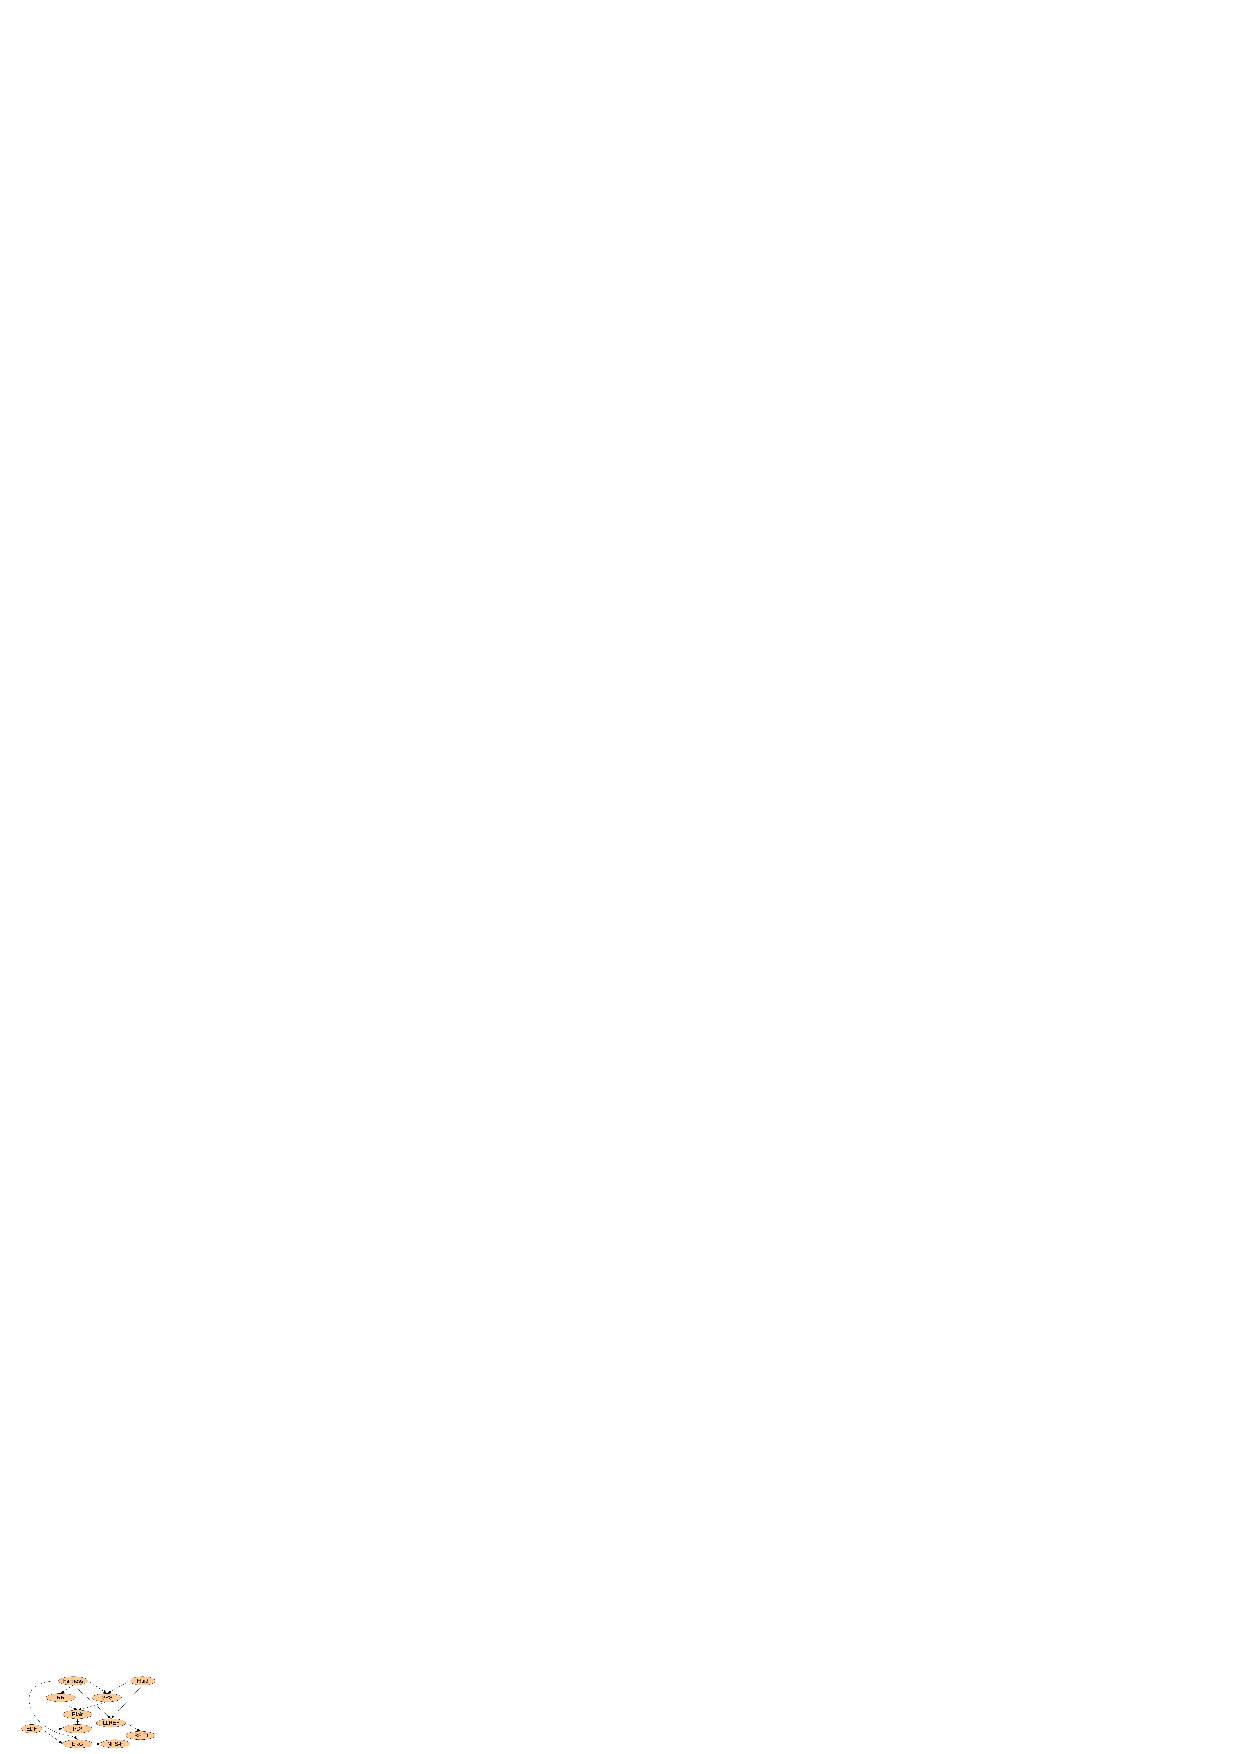
\includegraphics[width=10cm]{img/genealogy_pf}
\end{figure}
Ils précisent qu'\textit{EDF} n'est pas concerné par cette classification, mais qu'ayant 
inspiré certaines approches, il méritait de se trouver sur cette image. 
Nous invitons le lecteur intéressé par les influences des algorithmes entre eux 
à prendre connaissance de cet article extrêmement documenté.\\

De la lecture des articles, il ressort qu'une partie non négligeable d'entre eux 
est de parution récente, ce qui montre l'intérêt scientifique actuel pour ce type d'algorithmes. 
Bien évidemment, les propositions diffèrent par certaines propriétés. Par exemple, 
\textit{LB-Pfair} est orienté vers les systèmes critiques tolérants aux erreurs. 
Un enjeu très important de ce grand nombre d'algorithmes est de trouver une méthode qui 
garantisse l'optimalité pour la classe sporadique, tout en conservant de bonnes performances. 

La préoccupation principale actuelle est de trouver un moyen d'améliorer l'utilisation des processeurs (limitée à 
50\% pour les algorithmes partitionnés \cite{oh_utilization_1998}), sans détériorer les performances par 
une explosion du nombre de migrations, comme c'est généralement le cas avec des algorithmes globaux. 
Dans l'article d'Andersson de 2006 \cite{andersson_multiprocessor_2006}, la limite d'utilisation 
n'est pas aussi importante qu'avec une approche globale, mais le nombre de préemptions est limité par 
une constante $k$. En 2006 toujours, Cho et al. \cite{cho_optimal_2006} proposent \textit{LLREF} 
(largest local remaining execution time), dont l'optimalité est prouvée pour les 
systèmes périodiques. Ses performances ne sont à ce jour pas bien connues en pratique. %todo citer éventuellement 
% http://tesi.cab.unipd.it/51896/1/Implementation_and_Test_of_EDF_and_LLREF_Scgheduler_in_FreeRTOS.pdf
La liste proposée ici n'est pas exhaustive, un très grand nombre de propositions existe actuellement. 

\subsection{EDF-k}
%todo vérif la classe de tâches optimale pour EDF-k
En 2003, Goossens et al. proposent l'algorithme \textit{EDF-k} \cite{goossens_priority-driven_2003}, 
dont l'idée principale est d'être basé sur la priorité. 
La définition de \textit{Priority-driven Algorithm} (axé sur les priorités) 
est donnée par Ha et Liu en 1994 :
\begin{mydef}
	A Scheduling algorithm is said to be a priority driven scheduling algorithm if and 
	only if it satisfies the condition 
	that for every pair of jobs $J_i$ and $J_j$, if $J_i$ has a higher priority than $J_j$ at 
	some instant in time, then $J_i$ always has higher priority than $J_j$.
\end{mydef}
(Un algorithme d'ordonnancement est considéré comme axé sur les priorités si et seulement si il 
satisfait la condition suivante que pour chaque paire $J_i$ et $J_j$, si $J_i$ a une plus 
grande priorité que $J_j$ à un instant, $J_i$ a alors toujours une plus grande priorité 
que $J_j$.)\\
Suivant cette idée, \textit{EDF} est axé sur les priorités, là où \textit{PF} ne l'est pas.\\

Reprenant l'idée précédente de \textit{EDF-US} dont certaines tâches étaient de priorité 
supérieures, et d'autres de priorité simplement assignées par \textit{EDF} "classique", 
le nombre $k$ représente le nombre stable de tâches ($-1$) concernées par ces priorités 
supérieures. En d'autres termes, \textit{EDF-k} donne la priorité la plus élevée à 
$k - 1$ tâches, tandis que les autres sont ordonnancées suivant \textit{EDF}.\\

L'article propose une équation dont on dérive la valeur optimale de $k$, et où l'on peut 
atteindre $m$ le plus petit, cette valeur étant améliorée par rapport à \textit{EDF-US}.\\

Une autre approche consiste à considérer la laxité pour modifier \textit{EDF}. 
Ainsi, l'idée d'\textit{EDZL} (Earliest Deadline until Zero Laxity) \cite{cirinei_edzl_2007} ou encore d'EDCL \cite{kato_real-time_2007}
(Earliest Deadline Critical Laxity). \\

Des travaux récents continuent d'implémenter des versions d'\textit{EDF} avec stratégie 
globale, par exemple \textit{GEDF} \cite{li_global_2015}, donnant lieu à \textit{PGEDF}. Cette 
branche continue donc d'être étudiée et présente des intérêts.

\subsection{U-EDF}
\textit{U-EDF} est présenté en 2011 par Nelissen et al. \cite{nelissen_reducing_2011}. Il n'est pas "\textit{P-Fair}", et se démarque donc d'une bonne partie des algorithmes 
par le fait qu'il ne cherche pas à vérifier de condition de "P-équité".
Il prend en charge les systèmes périodiques à échéances implicites, et est optimal pour cette classe. 
Tout d'abord, la preuve de son optimalité se limite aux tâches périodiques dont on a dit plus haut qu'elles 
ne représentaient pas la majorité des classes e tâches des systèmes embarqués. 
En 2012, la preuve de son optimalité est élargie aux systèmes sporadiques par  Nelissen et al. \cite{nelissen_u-edf:_2012}. Le principal but de cet algorithme est de réduire le nombre de préemptions, 
ce qui est un grand inconvénient de l'approche globale. \\
L'idée principale d'\textit{U-EDF} est %todo add

\subsection{RUN}
Reduction to UNiprocessor (\textit{RUN}) est un algorithme présenté par Regnier et al. en 2013 \cite{regnier_multiprocessor_2013}. 
Cet algorithme est appliqué aux systèmes périodiques préemptifs à tâches indépendantes à 
échéances implicites. \textit{RUN} -- contrairement aux exemples vus précédemment -- n'applique pas 
la \textit{P-Fairness}, et parvient à réduire significativement le nombre de préemptions. 
\textit{RUN} réduit un ensemble de tâches en plus petits ensembles plus facilement ordonnançables 
en suivant deux opérations :\\
\begin{itemize}
    \item Une opération "\textit{Dual}"
    \item Une opération \textit{Pack}
\end{itemize}
Un \textit{Dual} se construit par complémentarité avec un \textit{Primal}, dont les règles de constructions sont 
données dans l'article.
Un serveur est chargé d'ordonnancer chaque sous-système. Celui-ci fonctionne à l'aide 
d'\textit{EDF}, dont les avantages nombreux ont déjà été évoqués plus tôt dans ce document. 
Il n'est pas évident à la lecture de l'article de comprendre en quoi 
diffère l'approche de \textit{RUN} par rapport à un ordonnanceur 
partitionné qui donnerait lieu à des systèmes ordonnancés à l'aide d'\textit{EDF}. 
En réalité, \textit{RUN} n'est pas un algorithme global, mais plutôt 
semi-partitionné, et la différence tient particulièrement du fait que les systèmes ne sont pas 
gérés par des processeurs distincts mais par des serveurs.  
Les auteurs insistent sur les avantages théoriques de RUN, qui devraient motiver une implémentation 
pratique afin de tester ses avantages. Cette implémentation a été faite 
\cite{compagnin_putting_2014} sur $LITMUS^{RT}$, et dont les résultats demandent à 
être confirmés mais montrent les bonnes performances sur ce système.\\

\textit{RUN} -- malgré son apparition récente -- a déjà des successeurs. \textit{QPS} est un algorithme 
également semi-partitionné, mais à la différence de RUN, il peut ordonnancer les systèmes 
de tâches indépendantes sporadiques à échéances implicites. 
Il est décrit dans un article de Massa et al. \cite{massa_outstanding_2014} en 2014. 
Comme pour \textit{RUN}, \textit{QPS} génère des sous-ensembles de tâches qui seront ordonnancés 
selon \textit{EDF} par des serveurs. Les auteurs présentent l'avantage d'une approche semi-partitionnée, 
qui fait un compromis entre les avantages de l'approche partitionnée et ceux de l'approche globale 
mais \textit{RUN} comporte quant à lui l'inconvénient de ne pas pouvoir s'appliquer aux tâches sporadiques. C'est ce qui explique la nécessité de l'existence de \textit{QPS}.

\subsection{Tableau comparatif des algorithmes globaux et semi-globaux}
Afin de faire le choix de l'algorithme à implémenter, une comparaison de ces algorithmes 
devrait être faite afin d'orienter le choix vers un ordonnanceur plutôt qu'un autre. 

\vspace{1em}

\begin{tabular}{|c|c|c|c|}
    \hline
    \textbf{Nom} & \textbf{Classe} &  \textbf{Optimal} & \textbf{Migrations}\\
    \hline
    \hline
    EDF-k & Sporadique, échéance implicite & Optimal (P-Fair) & Nombreuses \\
    \hline
    GEDF & Sporadique, échéance implicite & Non optimal & Nombreuses \\
    \hline    
    U-EDF & Sporadique, échéance implicite  & Optimal & Réduites\\
    \hline
    DP-WRAP & Sporadique, échéances arbitraires & Optimal (P-Fair)& Réduites\\
    \hline
    LLREF & Périodique, échéances arbitraires & Optimal & Réduites \\
    \hline
    BF & Périodiques, échéances implicites & Optimal & Réduites \\
    \hline
    RUN & Périodiques, échéances implicites & Optimal & Un peu réduites\\
    \hline
    QPS & Sporadiques, échéances arbitraires & Optimal & Réduites\\
    \hline
    
\end{tabular}


\section{Conclusion}
Nous avons exploré une petite partie de la littérature scientifique au sujet des ordonnanceurs 
globaux ou semi-partitionnés afin d'en sélectionner un pour implémentation et tests. 
Il ressort de cette étude que plusieurs candidats présentent des intérêts, sont mieux 
connus dans la littérature que dans la pratique, et gagneraient à être mieux analysés. 
Notre choix sera influencé par ces paramètres : \\
\begin{itemize}
    \item L'ordonnanceur est-il optimal
    \item Quels systèmes de tâche peut-il ordonnancer ?
    \item Des efforts ont-ils été fournis afin d'éviter les migrations ?
    \item A-t-il déjà bénéficié d'implémentations ?
\end{itemize}
De ces paramètres, il ressort que l'algorithme \textit{QPS} est optimal, semi-partitionné, 
peut ordonnancer les systèmes sporadiques à échéances arbitraires et 
les articles à son sujet parlent de bonnes performances concernant les migrations. \\
C'est donc vers cet algorithme que notre choix se porte.


\bibliographystyle{plain}
\bibliography{bibzotero}

\end{document}


